\documentclass[11pt]{article}

\usepackage[margin=1in]{geometry}
\usepackage{parskip}
\usepackage{titlesec}
\usepackage{enumitem}
\usepackage{graphicx}
\usepackage{booktabs}
\usepackage{float}
\usepackage{amsmath}

\titleformat{\section}{\normalfont\large\bfseries}{}{0em}{}
\titlespacing{\section}{0pt}{1.2em}{0.4em}
\titleformat{\subsection}{\normalfont\normalsize\bfseries}{}{0em}{}
\titlespacing{\subsection}{0pt}{0.9em}{0.3em}

\title{\vspace{-2em}Final Project, Part 1 --- Speed: The Cost of Execution Delay}
\author{Group 06\\ \small Alexandre Marthan, Elias Roubache, Elouan Bahri, Jean Jacob, Matthieu Pascal}
\date{\today}

\begin{document}
\maketitle
\vspace{-1em}

\noindent\textbf{Assets:} AAPL, GPRO, EUR/USD \quad\textbar\quad
\textbf{Period:} September 2019, 20 trading days \\
\textbf{Signals:} moving average and on-balance volume (paper), persistent quote imbalance (ours) \\
\textbf{Delays:} 0 ms, 100 ms, 1 s \quad\textbar\quad
\textbf{Book:} \$1{,}000{,}000

\section{Summary}

We apply the method of Scholtus and van Dijk (2012) to a liquid stock, a less
liquid stock and a currency pair. A trading signal is computed every minute and
the order it implies is executed 0 ms, 100 ms or 1 second later at the best bid
or ask of that moment. The question is how much return the delay costs.

\begin{enumerate}[leftmargin=1.6em, itemsep=0.25em]
  \item \textbf{All 27 strategies lose money once the spread is paid}, from
        $-0.19\%$ (EUR/USD, moving average) to $-109\%$ (GPRO, imbalance). On GPRO
        the three signals earn money at the mid quote, and the 22.5 bps spread
        takes it all back.
  \item \textbf{For one strategy over one month the cost of delay is too small to
        measure.} Averaged over the nine asset/signal pairs it is $+0.02\%$ at
        100 ms and $-0.12\%$ at 1 second, with a 90\% interval of $-0.42\%$ to
        $+0.14\%$.
  \item \textbf{Pooling the orders of a 601-rule universe makes it measurable, at
        1 second and not at 100 ms.} Executing 1 second late costs 0.07 bps per
        order for moving-average rules on AAPL, 0.06 bps for moving-average rules
        on GPRO and 0.11 bps for imbalance rules on GPRO. At 100 ms every effect
        is within 0.02 bps.
  \item \textbf{The paper's central result holds on the liquid stock, after its
        selection-bias test.} On AAPL, delay lowers the return of profitable rules
        by 0.7\% at 200 ms and 3.1\% at 1 second, more than random rules lose
        ($p = 0.03$ and $p < 0.001$). On GPRO and EUR/USD the losses at 1 second
        ($-1.0\%$ and $-1.2\%$) are what selection alone produces.
  \item \textbf{Tick frequency sets how often a delayed order meets a different
        quote} (62\% of the time after 1 second on AAPL, 55\% on EUR/USD, 1\% on
        GPRO); \textbf{tick size relative to price sets how much each miss costs}
        (22 bps on GPRO). Sensitivity to delay is the product of the two.
  \item \textbf{A \$1{,}000{,}000 order fills at the best quote only on EUR/USD.}
        It is half the displayed size there, 22 times the displayed size on AAPL
        and 53 times on GPRO.
\end{enumerate}

\section{What we implemented}

The assignment asks for two equities and one FX pair over one month, two signals
from the paper plus one of our own, three execution delays, the total return on a
\$1{,}000{,}000 book for each combination, and the cost of delay. The trading
procedure follows section 3.1 of the paper and the instructions of Discussion
Session 06.

\begin{itemize}[leftmargin=1.4em, itemsep=0.2em]
  \item \textbf{Signal.} Every 60 seconds a rule computes a position in
        $\{-1, 0, +1\}$ from the information available at the interval change.
  \item \textbf{Execution.} The order is executed a delay $d$ later against the
        best quote prevailing at that moment: buys pay the ask, sells receive the
        bid. The bid--ask spread is the only transaction cost.
  \item \textbf{Trading window.} Signals are acted upon from 09:40 to 15:50 New
        York time. The book is closed every day at the 15:50:00 price.
  \item \textbf{Size.} Every trade is for the number of units worth
        \$1{,}000{,}000 on the asset's first day: 4{,}850 AAPL shares, 263{,}505
        GPRO shares, EUR 913{,}013.
  \item \textbf{Return.} The total return of a strategy is the sum of the simple
        returns of its round trips, not compounded. For a long position entered at
        $t_1$ and closed at $t_2$, and for a short one,
        \[
          r^{\text{long}} = \frac{p^{bid}_{t_2+d} - p^{ask}_{t_1+d}}{p^{ask}_{t_1+d}},
          \qquad
          r^{\text{short}} = -\,\frac{p^{ask}_{t_2+d} - p^{bid}_{t_1+d}}{p^{bid}_{t_1+d}} .
        \]
        The dollar P\&L is the same sum valued on the fixed number of units.
  \item \textbf{Cost of delay.} Total return with delay $d$ minus total return
        with $d = 0$, for the same signal. \emph{Negative means the delay hurts.}
\end{itemize}

Three assets, three signals and three delays give 27 profit-and-loss reports: the
18 the assignment counts (three assets, the two signals taken from the paper,
three delays) and 9 for our own signal.

\section{Data and the three markets}

\textbf{Equities.} Databento Nasdaq TotalView-ITCH, MBP-1 schema: every trade and
every change of the best bid and offer, with nanosecond time stamps, from 09:30 to
16:00 New York time.

\textbf{EUR/USD.} Dukascopy tick data: every change of the best bid and ask with
the quoted sizes, with millisecond time stamps. The discussion session points to a
currency file on the MFE-4 server; we use a public source so that the FX leg covers
the same month, the same 20 days and the same clock window (13:30 to 20:00 UTC) as
the equities. The three assets then face the same number of signals.

\begin{table}[H]
  \centering
  \small
  \begin{tabular}{lrrr}
\toprule
Regular-session average & AAPL & GPRO & EUR/USD \\
\midrule
Mid price & $217.90$ & $4.51$ & $1.1011$ \\
Quoted spread (bps) & $0.73$ & $22.52$ & $0.27$ \\
One tick, in bps of the price & $0.46$ & $22.18$ & $0.09$ \\
One-minute volatility (bps) & $5.3$ & $17.0$ & $1.1$ \\
\midrule
Quote price changes per second & $8.80$ & $0.04$ & $1.21$ \\
Quote changed after 100 ms (\%) & $25.6$ & $0.2$ & $15.0$ \\
Quote changed after 1 s (\%) & $62.2$ & $1.1$ & $55.0$ \\
\midrule
Units in a \$1{,}000{,}000 order & $4{,}850$ & $263{,}505$ & $913{,}013$ \\
Units displayed at the best quote & $225$ & $4{,}945$ & $1{,}673{,}822$ \\
Order size / displayed size & $21.5$ & $53.3$ & $0.55$ \\
\bottomrule
\end{tabular}

  \caption{The three markets, September 2019. Units are shares for the stocks and
  euros for EUR/USD.}
  \label{tab:markets}
\end{table}

The three assets differ on three separate dimensions (Table~\ref{tab:markets}).

\begin{itemize}[leftmargin=1.4em, itemsep=0.2em]
  \item \textbf{Cost of trading.} EUR/USD is the cheapest (0.27 bps quoted
        spread) and AAPL is close behind (0.73 bps). GPRO is about 30 times more
        expensive than AAPL (22.5 bps): it trades near \$4.50, so the one-cent
        minimum tick alone is 22 bps of the price and its spread is pinned at one
        tick.
  \item \textbf{Tick frequency.} AAPL's best quote changes price 8.8 times per
        second, EUR/USD 1.2 times, GPRO once every 25 seconds. The quote a delayed
        order meets differs from the one the signal saw 62\% of the time after
        1 second on AAPL, 55\% on EUR/USD and 1.1\% on GPRO.
  \item \textbf{Size available.} The \$1{,}000{,}000 order is 22 times the size
        displayed at the best quote on AAPL and 53 times on GPRO, but only half of
        it on EUR/USD.
\end{itemize}

\textbf{Limits of the data.} The paper and the discussion session use a
price-impact price, the average price paid when the order walks the book. MBP-1
has no depth, so every order is assumed to fill in full at the best quote. The
last line of Table~\ref{tab:markets} shows that this is realistic for the currency
pair and optimistic for the two stocks. Under this assumption returns in percent
do not depend on the order size: they correspond to the paper's smallest capacity
level, and the dollar figures scale them to \$1{,}000{,}000. Spot FX has no public
trade tape, so the volume input of on-balance volume is tick volume for EUR/USD
(one unit for each quote that moves the mid). Dukascopy is one venue, so its tick
frequency understates the whole EUR/USD market.

\section{The three signals}

Inputs are sampled at each one-minute interval change $t$. Let $m_t$ be the mid
quote and $\overline{x}_t(n)$ the average of the last $n$ values of a series $x$.

\textbf{Moving average, MA (paper, eq.~3).} With a short window $s$, a long window
$l$ and a band $b$,
\[
  \text{MA}_t =
  \begin{cases}
    +1 & \text{if } \overline{m}_t(s) > (1+b)\,\overline{m}_t(l), \\
    -1 & \text{if } \overline{m}_t(s) < (1-b)\,\overline{m}_t(l), \\
    \phantom{+}0 & \text{otherwise.}
  \end{cases}
\]
Baseline: $s = 5$, $l = 30$, $b = 5$ bps, the smallest non-zero band of the paper's
grid, so that the rule also trades on EUR/USD.

\textbf{On-balance volume, OBV (paper, eq.~6).} The running sum since the open of
trade volume $v_j$ signed by the tick rule, auction crosses excluded:
\[
  obv_t = \sum_{j \le t} \operatorname{sign}(p_j - p_{j-1})\, v_j .
\]
The rule is long if $\overline{obv}_t(s) > \overline{obv}_t(l) + \text{band}$ and
short if $\overline{obv}_t(s) < \overline{obv}_t(l) - \text{band}$. Baseline:
$s = 5$, $l = 30$, $b = 0.5$. There are two departures from the paper. Volume is
added on an uptick and subtracted on a downtick, the standard convention; the
equation as printed in the paper has the opposite sign. And the paper's band is
proportional to the level of OBV; because OBV restarts at zero every day and
changes sign, our band is $b$ times the average one-minute volume over the long
window.

\textbf{Persistent quote imbalance, IMB (our own signal).} At every instant the
imbalance of the best quotes is
\[
  \frac{q^{bid} - q^{ask}}{q^{bid} + q^{ask}},
\]
with $q$ the size at the best bid and ask. $I_t$ is its time-weighted average over
the minute ending at $t$. The rule is long if $I > \theta$ in each of the last $k$
minutes, short if $I < -\theta$ in each of them, flat otherwise. Baseline: $k = 2$,
$\theta = 0.3$. The idea is that a queue that stays heavier on the bid for whole
minutes signals buying pressure that has not yet moved the price; requiring
persistence filters the flickering that dominates instantaneous imbalance.

\textbf{Parameters.} The baseline lookbacks and bands are values of the paper's
60-second settings (its Appendix~A). The same parameters are used for the three
assets and were not tuned to improve the P\&L. Lookback windows start at the 09:30
open, so the baseline MA and OBV give their first signal at 10:00 and IMB at 09:40.
The paper warms its rules up on pre-market quotes; we do not, because GPRO's
pre-market book is too thin to give a meaningful mid.

\textbf{Rule universe.} One rule per signal is enough for the 27 reports, but not
to measure an effect as small as the cost of delay. For that part we follow the
paper and use many rules: every combination of its 60-second grid for MA and OBV
(288 rules each) and 25 IMB rules, 601 rules per asset in total
(Appendix~A).

\section{The 27 profit-and-loss reports}

\begin{table}[H]
  \centering
  \resizebox{\textwidth}{!}{\begin{tabular}{llrrrrrrr}
\toprule
 & & & \multicolumn{3}{c}{Total return (\%)} & \multicolumn{3}{c}{P\&L (\$)} \\
\cmidrule(lr){4-6}\cmidrule(lr){7-9}
Asset & Signal & Trips & 0 ms & 100 ms & 1 s & 0 ms & 100 ms & 1 s \\
\midrule
AAPL & MA & $304$ & $-5.75$ & $-5.88$ & $-6.03$ & $-60{,}963$ & $-62{,}273$ & $-63{,}922$ \\
 & OBV & $103$ & $-0.89$ & $-0.81$ & $-0.90$ & $-9{,}603$ & $-8{,}827$ & $-9{,}700$ \\
 & IMB & $42$ & $-0.75$ & $-0.77$ & $-0.73$ & $-7{,}954$ & $-8{,}196$ & $-7{,}760$ \\
\midrule
GPRO & MA & $299$ & $-56.62$ & $-56.62$ & $-57.24$ & $-682{,}477$ & $-682{,}477$ & $-690{,}382$ \\
 & OBV & $150$ & $-26.52$ & $-26.52$ & $-26.10$ & $-310{,}935$ & $-310{,}935$ & $-305{,}665$ \\
 & IMB & $618$ & $-109.10$ & $-108.87$ & $-109.82$ & $-1{,}293{,}808$ & $-1{,}291{,}173$ & $-1{,}301{,}713$ \\
\midrule
EUR/USD & MA & $56$ & $-0.19$ & $-0.19$ & $-0.18$ & $-1{,}899$ & $-1{,}945$ & $-1{,}835$ \\
 & OBV & $158$ & $-1.48$ & $-1.45$ & $-1.36$ & $-14{,}846$ & $-14{,}617$ & $-13{,}695$ \\
 & IMB & $53$ & $-0.27$ & $-0.28$ & $-0.28$ & $-2{,}730$ & $-2{,}766$ & $-2{,}803$ \\
\bottomrule
\end{tabular}
}
  \caption{The 27 profit-and-loss reports. Total return is the sum of the simple
  round-trip returns; P\&L is in dollars for the fixed number of units.}
  \label{tab:pnl}
\end{table}

\begin{table}[H]
  \centering
  \resizebox{\textwidth}{!}{\begin{tabular}{llrrrrrrrr}
\toprule
Asset & Signal & P\&L at mid (\$) & Spread paid (\$) & Net bps / trip & Wins (\%) & Longs & Shorts & Holding (min) & Time in position (\%) \\
\midrule
AAPL & MA & $-37{,}878$ & $23{,}086$ & $-1.9$ & $33$ & $150$ & $154$ & $13.8$ & $57$ \\
 & OBV & $-1{,}334$ & $8{,}269$ & $-0.9$ & $42$ & $17$ & $86$ & $12.2$ & $17$ \\
 & IMB & $-4{,}971$ & $2{,}983$ & $-1.8$ & $31$ & $35$ & $7$ & $1.3$ & $1$ \\
\midrule
GPRO & MA & $+108{,}037$ & $790{,}514$ & $-18.9$ & $18$ & $156$ & $143$ & $19.1$ & $77$ \\
 & OBV & $+84{,}321$ & $395{,}257$ & $-17.7$ & $17$ & $69$ & $81$ & $10.7$ & $22$ \\
 & IMB & $+339{,}921$ & $1{,}633{,}729$ & $-17.7$ & $9$ & $360$ & $258$ & $3.8$ & $32$ \\
\midrule
EUR/USD & MA & $-347$ & $1{,}552$ & $-0.3$ & $27$ & $30$ & $26$ & $9.8$ & $7$ \\
 & OBV & $-10{,}564$ & $4{,}282$ & $-0.9$ & $23$ & $85$ & $73$ & $9.6$ & $20$ \\
 & IMB & $-1{,}516$ & $1{,}214$ & $-0.5$ & $25$ & $25$ & $28$ & $1.8$ & $1$ \\
\bottomrule
\end{tabular}
}
  \caption{Where the P\&L comes from, with instantaneous execution. \emph{P\&L at
  mid} values the same trades at the mid quote, so \emph{Spread paid} is the
  difference with the actual P\&L. \emph{Holding} is the average length of a
  position.}
  \label{tab:decomp}
\end{table}

\begin{itemize}[leftmargin=1.4em, itemsep=0.2em]
  \item \textbf{Every strategy loses money net of the spread}
        (Table~\ref{tab:pnl}). Total returns range from $-0.19\%$ (EUR/USD, MA,
        56 round trips) to $-109\%$ (GPRO, IMB, 618 round trips). A book below zero
        is possible because the same number of units is traded on every signal
        without compounding: 618 round trips at about 18 bps each cost more than
        the book. The paper studies speed, not profitability, and most of its
        rules lose as well (58\% of those that trade on a given day).
  \item \textbf{On GPRO the loss is the spread} (Table~\ref{tab:decomp}). Valued
        at the mid, the three GPRO strategies make money: $+\$108{,}037$ for MA,
        $+\$84{,}321$ for OBV and $+\$339{,}921$ for IMB. The spread paid is \$0.4
        to \$1.6 million. The signals predict the direction of the next move, but
        not by the 22.5 bps a round trip costs.
  \item \textbf{On AAPL the signal itself loses.} AAPL MA loses \$37{,}878 at the
        mid out of \$60{,}963 in total: a trend rule on one-minute mids buys after
        the rise and the price partly reverts. The spread is a secondary cost
        there.
  \item \textbf{Holding times.} MA positions last 10 to 19 minutes on average, OBV
        positions 10 to 12 minutes, IMB positions 1 to 4 minutes. MA trades about
        300 times on each stock and 56 times on EUR/USD, whose one-minute
        volatility (1.1 bps) rarely carries the short average 5 bps away from the
        long one. IMB trades far more on GPRO (618 round trips) than on AAPL (42)
        or EUR/USD (53): GPRO's queues are large and persistently one-sided.
  \item \textbf{The three delay columns are almost identical.} For each strategy
        the delays differ by far less than the strategy loses.
\end{itemize}

\section{Cost of delay of the nine strategies}

Table~\ref{tab:cost} gives the cost of delay at the two required delays, with two
measures of uncertainty: the Wilcoxon signed-rank test on the 20 daily differences,
which is the paper's test, and a 90\% interval obtained by resampling the 20
trading days 5{,}000 times. Figure~\ref{fig:curve} extends the delays to the whole
range from 0 to 1{,}000 ms.

\begin{table}[H]
  \centering
  \resizebox{\textwidth}{!}{\begin{tabular}{llrlrlrr}
\toprule
 & & \multicolumn{2}{c}{100 ms} & \multicolumn{4}{c}{1 second} \\
\cmidrule(lr){3-4}\cmidrule(lr){5-8}
Asset & Signal & Cost (\%) & 90\% interval & Cost (\%) & 90\% interval & Cost (\$) & Wilcoxon $p$ \\
\midrule
AAPL & MA & $-0.12$ & [$-0.39$, $0.09$] & $-0.27$ & [$-0.80$, $0.26$] & $-2{,}958$ & $0.37$ \\
 & OBV & $+0.07$ & [$0.01$, $0.14$] & $-0.01$ & [$-0.20$, $0.18$] & $-97$ & $0.90$ \\
 & IMB & $-0.02$ & [$-0.08$, $0.02$] & $+0.02$ & [$-0.05$, $0.09$] & $+194$ & $0.54$ \\
\midrule
GPRO & MA & $0.00$ & [$-0.44$, $0.44$] & $-0.62$ & [$-2.31$, $0.68$] & $-7{,}905$ & $0.81$ \\
 & OBV & $0.00$ & [$0.00$, $0.00$] & $+0.42$ & [$0.00$, $0.87$] & $+5{,}270$ & n/a \\
 & IMB & $+0.23$ & [$-0.40$, $0.86$] & $-0.72$ & [$-2.16$, $0.57$] & $-7{,}905$ & $0.28$ \\
\midrule
EUR/USD & MA & $-0.005$ & [$-0.015$, $0.007$] & $+0.006$ & [$-0.026$, $0.043$] & $+64$ & $0.85$ \\
 & OBV & $+0.023$ & [$0.002$, $0.053$] & $+0.115$ & [$-0.015$, $0.322$] & $+1{,}150$ & $0.57$ \\
 & IMB & $-0.004$ & [$-0.007$, $-0.001$] & $-0.007$ & [$-0.026$, $0.013$] & $-73$ & $0.45$ \\
\midrule
\multicolumn{2}{l}{Mean of the nine} & $+0.02$ & [$-0.07$, $0.10$] & $-0.12$ & [$-0.42$, $0.14$] &  &  \\
\bottomrule
\end{tabular}
}
  \caption{Cost of delay of the nine strategies: total return with the delay minus
  total return at 0 ms, in percentage points. Negative means the delay hurts. The
  Wilcoxon test is not reported when fewer than six days differ.}
  \label{tab:cost}
\end{table}

\begin{figure}[H]
  \centering
  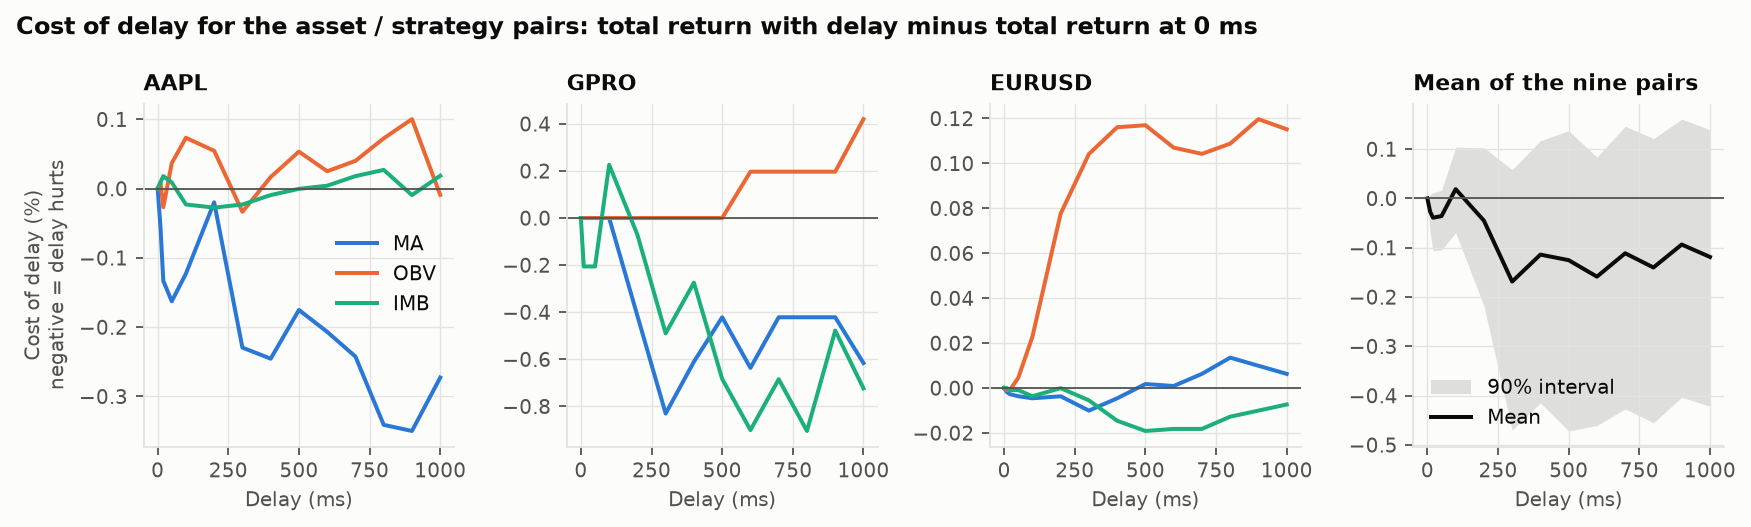
\includegraphics[width=\textwidth]{figures/03_cost_of_delay_curve.png}
  \caption{Cost of delay from 0 to 1{,}000 ms for each asset and signal, and mean of
  the nine pairs with its 90\% interval.}
  \label{fig:curve}
\end{figure}

\begin{itemize}[leftmargin=1.4em, itemsep=0.2em]
  \item \textbf{At 100 ms the cost is within 0.23 percentage points for all nine
        pairs}, with no consistent sign: negative for AAPL MA ($-0.12\%$), positive
        for GPRO IMB ($+0.23\%$) and AAPL OBV ($+0.07\%$), zero for GPRO MA and
        OBV, whose execution prices almost never change within 100 ms. The mean
        over the nine pairs is $+0.02\%$.
  \item \textbf{At 1 second the less liquid stock pays the most.} GPRO IMB loses
        0.72 percentage points and GPRO MA 0.62 ($-\$7{,}905$ each). AAPL MA loses
        0.27 ($-\$2{,}958$) and EUR/USD MA is unchanged.
  \item \textbf{The OBV strategies gain from delay} at 1 second on GPRO
        ($+0.42\%$) and EUR/USD ($+0.12\%$).
  \item \textbf{The mean curve is negative at every delay from 200 ms}, between
        $-0.05\%$ and $-0.17\%$, and stands at $-0.12\%$ at 1 second. This is the
        shape of the discussion-session example: a small, noisy effect at short
        delays, a steady cost at longer ones.
  \item \textbf{None of this is statistically distinguishable from zero.} The 90\%
        interval of the mean is $-0.42\%$ to $+0.14\%$ at 1 second, and every
        1-second interval in Table~\ref{tab:cost} contains zero or touches it. The
        only intervals that exclude zero are three small effects at 100 ms. On
        GPRO a single one-cent difference on one execution moves the total return
        by 0.22\%.
\end{itemize}

One strategy over one month places 84 to 1{,}236 orders. That is not enough to
measure an effect of a few hundredths of a basis point per order, which is why the
paper works with thousands of rules. The next section does the same.

\section{Importance of speed over a 601-rule universe}

\subsection{All rules (Figure 6 of the paper)}

As in the paper, each day the average return across rules with delay $d$ is
compared with the average under instantaneous execution, in percent of the latter,
and the daily figures are averaged over the 20 days. Rules with a zero return on a
day are excluded; on an average day 414 rules trade on AAPL, 547 on GPRO and 303
on EUR/USD.

\begin{table}[H]
  \centering
  \small
  \begin{tabular}{lrrrrr}
\toprule
Asset & Delay (ms) & Mean of daily ratios (\%) & Median (\%) & Bps per rule-day & Wilcoxon $p$ \\
\midrule
AAPL & $100$ & $+1.23$ & $+0.10$ & $0.00$ & $0.60$ \\
 & $200$ & $+1.37$ & $+0.13$ & $-0.08$ & $0.93$ \\
 & $500$ & $+3.09$ & $-1.10$ & $-0.32$ & $0.35$ \\
 & $1{,}000$ & $+0.92$ & $-2.26$ & $-0.77$ & $0.064$ \\
\midrule
GPRO & $100$ & $-0.10$ & $0.00$ & $-0.16$ & $0.64$ \\
 & $200$ & $-0.19$ & $0.00$ & $-0.29$ & $0.28$ \\
 & $500$ & $-0.15$ & $0.00$ & $-0.21$ & $0.84$ \\
 & $1{,}000$ & $-0.49$ & $-0.58$ & $-0.86$ & $0.11$ \\
\midrule
EUR/USD & $100$ & $-0.90$ & $+0.08$ & $+0.01$ & $0.81$ \\
 & $200$ & $+3.74$ & $+0.56$ & $+0.08$ & $0.004$ \\
 & $500$ & $+3.53$ & $+1.06$ & $+0.12$ & $0.004$ \\
 & $1{,}000$ & $+3.15$ & $+2.43$ & $+0.17$ & $0.002$ \\
\bottomrule
\end{tabular}

  \caption{Importance of speed for all rules. The first column is the paper's
  statistic (mean over days of the relative change in the average return); the
  second is the median of the same daily figures; the third is the change in the
  average return in bps per rule-day, which does not depend on a ratio, with its
  Wilcoxon test.}
  \label{tab:fig6}
\end{table}

\begin{itemize}[leftmargin=1.4em, itemsep=0.2em]
  \item \textbf{At 100 ms nothing is distinguishable from zero} on any asset.
  \item \textbf{GPRO declines with delay}: $-0.10\%$ at 100 ms and $-0.49\%$ at
        1 second, or 0.86 bps per rule-day ($p = 0.11$).
  \item \textbf{AAPL loses at 1 second, but the paper's statistic hides it.} The
        mean of daily ratios is positive ($+0.9\%$) because a few days on which
        the average return is close to zero dominate it. The median is $-2.3\%$,
        and in return terms a 1 second delay costs 0.77 bps per rule-day
        ($p = 0.06$).
  \item \textbf{On EUR/USD delay helps from 200 ms}: $+0.17$ bps per rule-day at
        1 second ($p = 0.002$).
\end{itemize}

These averages mix rules that make money with rules that lose money. The paper
shows that the two behave differently, and warns that separating them creates a
bias.

\subsection{Winning and losing rules, and the selection bias (Figure 7 of the paper)}

Selecting the rules with a positive return at 0 ms selects trades whose first
instants went well. Delaying them removes part of that return mechanically, even if
the signal contains no information. The paper measures this selection bias by
applying the signals generated on one day to the prices of another, random day:
these random rules trade as often and hold as long as the real ones but know
nothing about the day they trade. We do the same 5{,}000 times. An actual value
below the 5th percentile of the random rules is a loss that selection cannot
explain: a one-sided test at the 5\% level, as in the paper.

\begin{figure}[H]
  \centering
  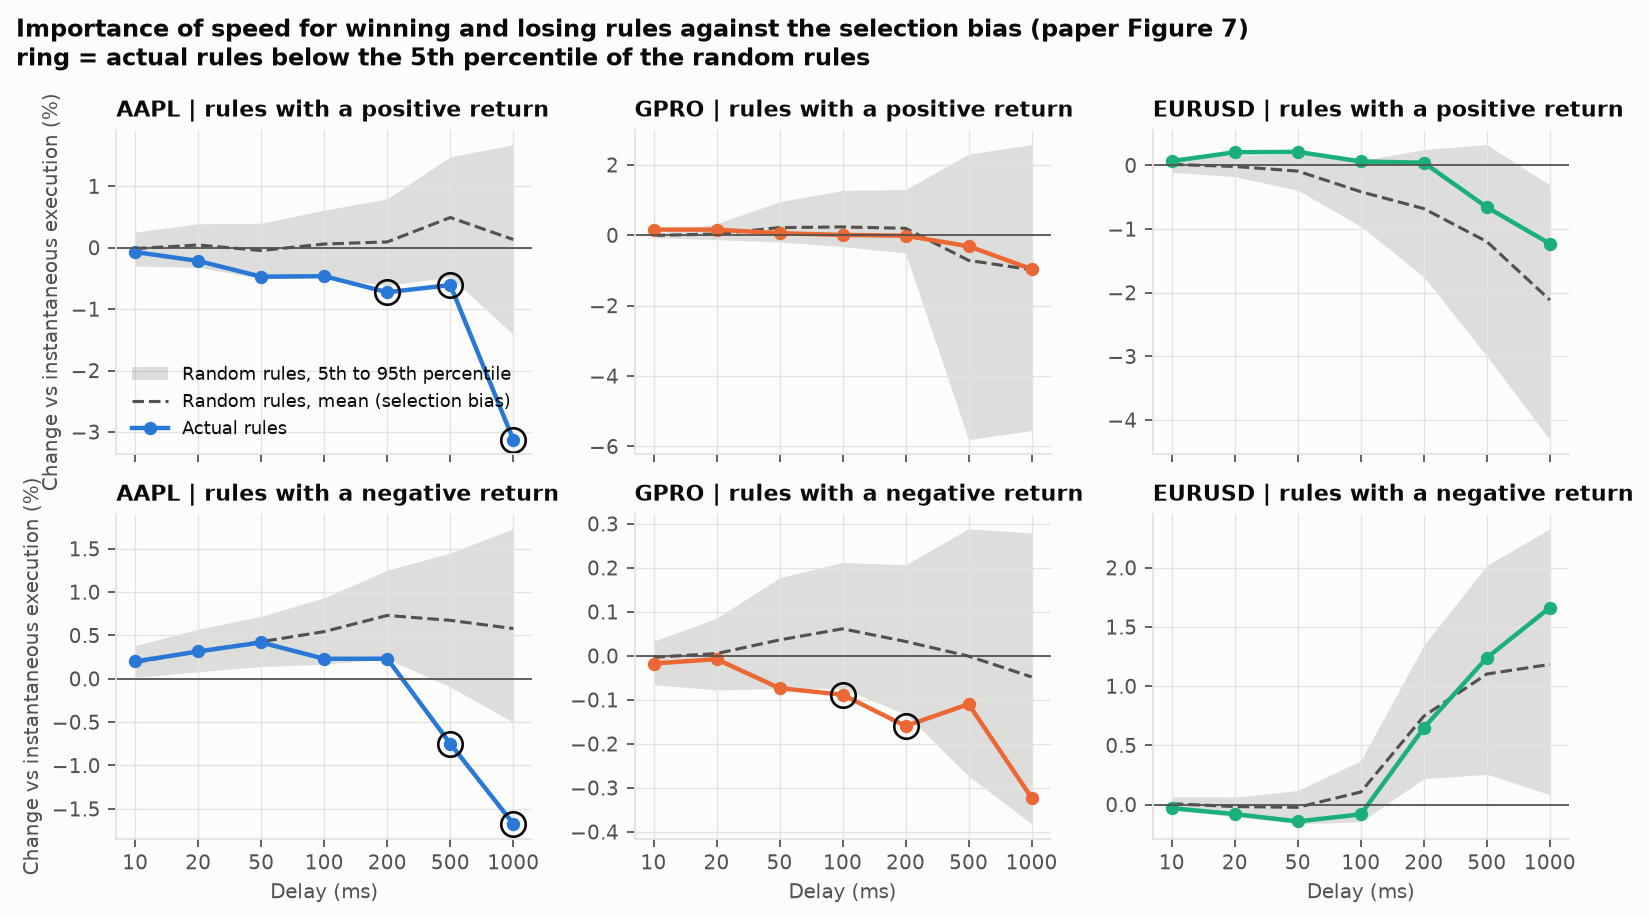
\includegraphics[width=\textwidth]{figures/05_importance_of_speed_selection_bias.png}
  \caption{Importance of speed for rules with a positive (top) and negative
  (bottom) return at 0 ms. Dashed line: mean of the random rules, which is the
  selection bias. Band: their 5th to 95th percentile. Ring: actual rules below the
  band.}
  \label{fig:selection}
\end{figure}

\begin{table}[H]
  \centering
  \resizebox{\textwidth}{!}{\begin{tabular}{lrrlrrlrrlr}
\toprule
 & & \multicolumn{3}{c}{AAPL} & \multicolumn{3}{c}{GPRO} & \multicolumn{3}{c}{EUR/USD} \\
\cmidrule(lr){3-5}\cmidrule(lr){6-8}\cmidrule(lr){9-11}
 & Delay (ms) & Actual (\%) & Random rules & $p$ & Actual (\%) & Random rules & $p$ & Actual (\%) & Random rules & $p$ \\
\midrule
Winning rules & $100$ & $-0.46$ & [$-0.49$, $0.61$] & $0.058$ & $+0.01$ & [$-0.32$, $1.27$] & $0.42$ & $+0.06$ & [$-0.96$, $0.07$] & $0.94$ \\
 & $200$ & $-0.73$* & [$-0.61$, $0.80$] & $0.034$ & $-0.01$ & [$-0.51$, $1.30$] & $0.39$ & $+0.04$ & [$-1.75$, $0.25$] & $0.89$ \\
 & $500$ & $-0.61$* & [$-0.48$, $1.48$] & $0.030$ & $-0.31$ & [$-5.81$, $2.30$] & $0.54$ & $-0.66$ & [$-3.00$, $0.32$] & $0.69$ \\
 & $1{,}000$ & $-3.13$* & [$-1.41$, $1.68$] & $<0.001$ & $-0.96$ & [$-5.55$, $2.57$] & $0.47$ & $-1.23$ & [$-4.31$, $-0.31$] & $0.76$ \\
\midrule
Losing rules & $100$ & $+0.23$ & [$0.17$, $0.93$] & $0.091$ & $-0.09$* & [$-0.07$, $0.21$] & $0.034$ & $-0.08$ & [$-0.15$, $0.37$] & $0.11$ \\
 & $200$ & $+0.23$ & [$0.23$, $1.25$] & $0.052$ & $-0.16$* & [$-0.13$, $0.21$] & $0.033$ & $+0.65$ & [$0.22$, $1.34$] & $0.41$ \\
 & $500$ & $-0.75$* & [$-0.09$, $1.45$] & $0.001$ & $-0.11$ & [$-0.27$, $0.29$] & $0.27$ & $+1.24$ & [$0.26$, $2.02$] & $0.62$ \\
 & $1{,}000$ & $-1.67$* & [$-0.50$, $1.73$] & $<0.001$ & $-0.32$ & [$-0.38$, $0.28$] & $0.087$ & $+1.66$ & [$0.08$, $2.33$] & $0.76$ \\
\bottomrule
\end{tabular}
}
  \caption{Importance of speed (\%) for winning and losing rules. \emph{Random
  rules} is the 5th to 95th percentile of the same statistic for the random rules;
  $p$ is the share of the 5{,}000 draws at or below the actual value. A star marks
  $p < 0.05$.}
  \label{tab:selection}
\end{table}

\begin{itemize}[leftmargin=1.4em, itemsep=0.2em]
  \item \textbf{AAPL, winning rules: speed matters.} Delay lowers the return of
        profitable rules by 0.5\% at 100 ms, 0.7\% at 200 ms and 3.1\% at
        1 second. Random rules lose nothing ($+0.1\%$ at 1 second, band $-1.4\%$ to
        $+1.7\%$), so this is not a selection effect: $p = 0.06$ at 100 ms, $0.03$
        at 200 ms and at 500 ms, below $0.001$ at 1 second. This is the paper's
        main result, with the same threshold of about 200 ms.
  \item \textbf{AAPL, losing rules.} Up to 200 ms they behave like random rules. At
        500 ms and 1 second they lose more ($-1.7\%$ at 1 second against $+0.6\%$
        for random rules, $p < 0.001$). The paper finds no effect of speed on
        losing rules; on AAPL a 1 second delay hurts whatever the rule's result.
  \item \textbf{GPRO, winning rules: no evidence.} The $-1.0\%$ at 1 second equals
        the selection bias ($-1.0\%$, band $-5.5\%$ to $+2.6\%$). Only 67 rules a
        day make money on GPRO, 12\% of those that trade, so the band is wide.
        Losing rules lose slightly more than random ones at 100 and 200 ms
        ($-0.09\%$ and $-0.16\%$, $p = 0.03$).
  \item \textbf{EUR/USD: the raw numbers are selection.} Winning rules lose 1.2\%
        at 1 second, but random rules lose 2.1\% (band $-4.3\%$ to $-0.3\%$).
        Losing rules gain 1.7\%, and random ones gain 1.2\%. Neither is evidence of
        an effect of speed.
\end{itemize}

Without the random rules we would have concluded that delay hurts winning rules on
all three assets. Beyond selection, it only does on the liquid stock.

\subsection{Comparison with the paper}

\begin{table}[H]
  \centering
  \small
  \begin{tabular}{rrrrrrr}
\toprule
 & \multicolumn{3}{c}{Paper, January to September 2009} & \multicolumn{3}{c}{This project, September 2019} \\
\cmidrule(lr){2-4}\cmidrule(lr){5-7}
Delay (ms) & SPY & QQQQ & IWM & AAPL & GPRO & EUR/USD \\
\midrule
$100$ & $-0.07$ & $-0.07$ & $-0.07$ & $-0.46$ & $+0.01$ & $+0.06$ \\
$200$ & $-0.22$* & $-0.26$ & $-0.15$ & $-0.73$* & $-0.01$ & $+0.04$ \\
$500$ & $-0.39$* & $-1.01$* & $-0.62$* & $-0.61$* & $-0.31$ & $-0.66$ \\
$1{,}000$ & $-1.05$* & $-1.91$* & $-1.34$* & $-3.13$* & $-0.96$ & $-1.23$ \\
\bottomrule
\end{tabular}

  \caption{Importance of speed (\%) for rules with a positive return, 60-second
  signals. Paper: Table B.1 of its internet appendix (186 trading days, 27{,}424
  rules, orders of 100 shares). A star marks a loss that is significant against the
  selection bias.}
  \label{tab:paper}
\end{table}

The liquid stock reproduces the paper (Table~\ref{tab:paper}): no significant
effect at 100 ms, a significant loss from 200 ms, and a loss at 1 second
($-3.1\%$) of the same order as the paper's ETFs ($-1.0\%$ to $-1.9\%$), somewhat
larger. Ten years later, and on a single stock instead of an index ETF, the
importance of speed has the same shape. The less liquid stock and the currency
pair show losses of a similar size at 1 second, which 20 days cannot separate from
the selection bias.

\subsection{Effect of the delay per order}

The split between winning and losing rules conditions on performance. The
following measure does not. For every order of every rule, the effect of executing
it $h$ later is
\[
  e_h = -\,\delta\;\frac{p_{t+h} - p_t}{p_t},
\]
with $\delta = +1$ and $p$ the ask for a buy, $\delta = -1$ and $p$ the bid for a
sell. It is negative when the price moves in the direction of the order during the
delay. Summed over the orders of a strategy it is that strategy's cost of delay,
so this is the same quantity measured order by order. Pooling the 601 rules gives
9{,}000 to 120{,}000 orders per signal family and asset. The 90\% intervals
resample trading days, which preserves the dependence between rules that trade at
the same instant.

\begin{table}[H]
  \centering
  \resizebox{\textwidth}{!}{\begin{tabular}{llrrlrl}
\toprule
 & & & \multicolumn{2}{c}{100 ms} & \multicolumn{2}{c}{1 second} \\
\cmidrule(lr){4-5}\cmidrule(lr){6-7}
Asset & Signal & Orders & Bps / order & 90\% interval & Bps / order & 90\% interval \\
\midrule
AAPL & MA & $83{,}616$ & $-0.002$ & [$-0.012$, $0.007$] & $-0.070$* & [$-0.113$, $-0.032$] \\
 & OBV & $59{,}390$ & $-0.001$ & [$-0.013$, $0.010$] & $-0.027$ & [$-0.074$, $0.012$] \\
 & IMB & $11{,}702$ & $+0.006$ & [$0.000$, $0.011$] & $+0.015$ & [$-0.009$, $0.037$] \\
\midrule
GPRO & MA & $121{,}602$ & $-0.006$ & [$-0.025$, $0.010$] & $-0.058$* & [$-0.109$, $-0.007$] \\
 & OBV & $78{,}714$ & $-0.007$ & [$-0.031$, $0.017$] & $+0.003$ & [$-0.045$, $0.056$] \\
 & IMB & $25{,}622$ & $-0.017$ & [$-0.043$, $0.005$] & $-0.107$* & [$-0.180$, $-0.040$] \\
\midrule
EUR/USD & MA & $39{,}138$ & $-0.0005$ & [$-0.0019$, $0.0009$] & $+0.0029$ & [$-0.0026$, $0.0086$] \\
 & OBV & $90{,}128$ & $+0.0010$ & [$-0.0002$, $0.0023$] & $+0.0104$* & [$0.0061$, $0.0151$] \\
 & IMB & $9{,}438$ & $-0.0011$* & [$-0.0020$, $-0.0003$] & $-0.0021$ & [$-0.0058$, $0.0016$] \\
\bottomrule
\end{tabular}
}
  \caption{Effect of the delay per order, in bps of the price, over the rule
  universe. Negative means the delay hurts. A star marks a 90\% interval that
  excludes zero. \emph{Return at 0 ms} is the average return of the family's rules
  in bps per rule-day.}
  \label{tab:order}
\end{table}

\begin{figure}[H]
  \centering
  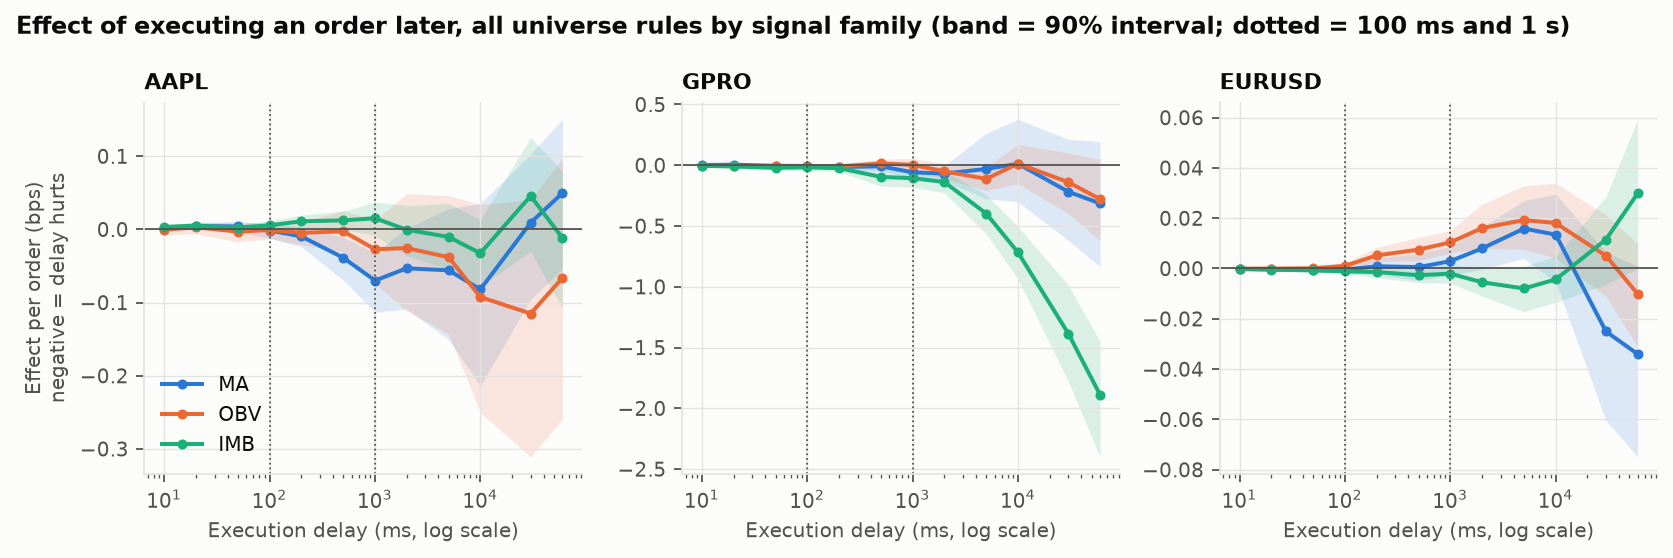
\includegraphics[width=\textwidth]{figures/06_order_response_curve.png}
  \caption{Effect of executing an order later, from 10 ms to 60 seconds, by signal
  family. Bands are 90\% intervals.}
  \label{fig:response}
\end{figure}

\begin{itemize}[leftmargin=1.4em, itemsep=0.2em]
  \item \textbf{100 ms costs nothing measurable.} Every family on every asset is
        within 0.02 bps per order, and only one interval excludes zero (EUR/USD
        IMB, $-0.001$ bps).
  \item \textbf{1 second has a cost on the two stocks} (Table~\ref{tab:order}):
        0.07 bps per order for MA rules on AAPL, 0.06 bps for MA rules on GPRO and
        0.11 bps for IMB rules on GPRO.
  \item \textbf{The cost is the signal's short-run predictive power}
        (Figure~\ref{fig:response}). After an IMB order on GPRO the price keeps
        moving in the order's direction: 0.4 bps after 5 seconds, 1.9 bps after
        60 seconds. The signal predicts the next minute, and each second of delay
        gives up a slice of that move. On AAPL the drift after MA orders builds up
        over the first second (0.04 bps at 500 ms, 0.07 at 1 second) and is gone
        after 30 seconds.
  \item \textbf{On EUR/USD delay helps OBV rules}, by 0.01 bps per order at
        1 second: the price moves back after their orders. The amount is 4\% of
        the spread.
  \item \textbf{Relative to the spread the cost is small.} 0.07 bps is 19\% of
        AAPL's half-spread; 0.11 bps is 1\% of GPRO's.
\end{itemize}

\section{Answers to the three questions of the assignment}

\subsection{(a) Is one asset affected more or less by execution delays, and why?}

\textbf{The two stocks are affected at 1 second; the currency pair is not; nothing
is affected at 100 ms.}

\begin{itemize}[leftmargin=1.4em, itemsep=0.2em]
  \item \textbf{AAPL is the asset where speed matters most clearly.} Its book
        changes 8.8 times per second, so a delayed order usually meets a different
        quote, and a one-cent move is worth more than its half-spread. The cost is
        significant from 200 ms for profitable rules.
  \item \textbf{GPRO pays the most in percent for a single strategy.} Its MA and
        IMB strategies lose 0.6\% and 0.7\% at 1 second, against 0.3\% for AAPL's
        MA, because each change of its quote is a full tick of 22 bps. But its
        quote changes so rarely that the cost comes from a handful of executions,
        and it is not statistically measurable for one strategy.
  \item \textbf{EUR/USD is not affected.} Its ticks are frequent but tiny (under
        0.1 bp), and its one-minute signals have no short-run predictive power to
        lose.
\end{itemize}

A delay costs money when two conditions hold: the quote moves during the delay,
and it moves in the direction of the order, which requires a signal that predicts
the next move. On AAPL both hold within a second for the MA rules. On GPRO the
quote rarely moves, but the imbalance signal predicts its direction when it does.
On EUR/USD the quote moves often, by very little, and not in the direction of the
orders.

\subsection{(b) Do the signals perform differently under certain market conditions?}

Days are split, asset by asset, into the 10 most and 10 least volatile, by
one-minute mid-quote volatility (Table~\ref{tab:regimes}).

\begin{table}[H]
  \centering
  \small
  \begin{tabular}{llrrrrrr}
\toprule
 & & \multicolumn{2}{c}{Return at 0 ms} & \multicolumn{2}{c}{Cost of 1 s} & \multicolumn{2}{c}{Effect of 1 s per order} \\
 & & \multicolumn{2}{c}{(bps / rule-day)} & \multicolumn{2}{c}{(bps / rule-day)} & \multicolumn{2}{c}{(bps)} \\
\cmidrule(lr){3-4}\cmidrule(lr){5-6}\cmidrule(lr){7-8}
Asset & Signal & High vol & Low vol & High vol & Low vol & High vol & Low vol \\
\midrule
AAPL & MA & $-27.4$ & $-18.6$ & $-2.14$ & $-0.34$ & $-0.111$ & $-0.017$ \\
 & OBV & $-9.7$ & $-11.2$ & $-1.27$ & $+0.44$ & $-0.080$ & $+0.027$ \\
 & IMB & $-9.8$ & $-18.2$ & $-0.13$ & $+1.43$ & $-0.003$ & $+0.032$ \\
\midrule
GPRO & MA & $-256.1$ & $-246.1$ & $-3.16$ & $+0.65$ & $-0.135$ & $+0.032$ \\
 & OBV & $-157.3$ & $-161.4$ & $+0.07$ & $+0.02$ & $+0.004$ & $+0.001$ \\
 & IMB & $-517.7$ & $-406.0$ & $-9.70$ & $-1.40$ & $-0.174$ & $-0.029$ \\
\midrule
EUR/USD & MA & $-5.1$ & $-7.3$ & $+0.05$ & $+0.08$ & $+0.0027$ & $+0.0032$ \\
 & OBV & $-9.1$ & $-7.6$ & $+0.33$ & $+0.15$ & $+0.0137$ & $+0.0069$ \\
 & IMB & $-5.8$ & $-6.4$ & $-0.13$ & $-0.01$ & $-0.0039$ & $-0.0002$ \\
\bottomrule
\end{tabular}

  \caption{Signals across volatility regimes, over the rule universe. Costs and
  effects are negative when the delay hurts.}
  \label{tab:regimes}
\end{table}

\begin{itemize}[leftmargin=1.4em, itemsep=0.2em]
  \item \textbf{The cost of delay is concentrated on volatile days.} MA rules lose
        0.11 bps per order to a 1 second delay on AAPL's volatile days against 0.02
        on quiet days, and 0.14 against a small gain on GPRO. IMB on GPRO loses
        0.17 bps per order on volatile days against 0.03. The quote moves further
        during the delay when the market moves faster.
  \item \textbf{OBV changes sign.} On AAPL a 1 second delay costs OBV rules
        0.08 bps per order on volatile days and helps them by 0.03 on quiet days.
        On GPRO it shows nothing in either regime.
  \item \textbf{Performance itself depends on the regime.} MA rules on AAPL lose
        more on volatile days ($-27$ against $-19$ bps per rule-day): the band is
        crossed more often and reversed more often. IMB on AAPL loses less on
        volatile days ($-10$ against $-18$). IMB on GPRO loses more ($-518$ against
        $-406$), because it trades more and pays the spread each time.
  \item \textbf{This differs from the paper}, which finds that speed matters more
        on low-volatility days for SPY.
\end{itemize}

\subsection{(c) Does tick frequency affect the importance of delays, and how would we factor it in?}

\begin{table}[H]
  \centering
  \small
  \begin{tabular}{lrrr}
\toprule
 & AAPL & GPRO & EUR/USD \\
\midrule
Quote price changes per second & $8.80$ & $0.04$ & $1.21$ \\
Quote changed after 100 ms / 1 s (\%) & $25.6$ / $62.2$ & $0.2$ / $1.1$ & $15.0$ / $55.0$ \\
Mean absolute mid move after 1 s (bps) & $0.48$ & $0.24$ & $0.08$ \\
\quad in half-spreads & $1.31$ & $0.02$ & $0.62$ \\
\midrule
Absolute effect of 100 ms per round trip (bps) & $0.12$ & $0.08$ & $0.01$ \\
Absolute effect of 1 s per round trip (bps) & $0.38$ & $0.42$ & $0.07$ \\
\midrule
Correlation of daily sensitivity with quote changes & $0.48$ & $0.57$ & $0.55$ \\
Correlation of daily sensitivity with volatility & $0.48$ & $0.69$ & $0.67$ \\
\bottomrule
\end{tabular}

  \caption{Tick frequency and sensitivity to delay. The absolute effect is the mean
  absolute change in return caused by the delay, per round trip, over the rule
  universe; it measures sensitivity regardless of sign.}
  \label{tab:tick}
\end{table}

\textbf{Partly: tick frequency sets the probability of a stale quote, and tick
size sets what a stale quote costs} (Table~\ref{tab:tick}).

\begin{itemize}[leftmargin=1.4em, itemsep=0.2em]
  \item \textbf{At 100 ms the fast book is the most exposed}: the absolute effect
        per round trip is 0.12 bps on AAPL, against 0.08 on GPRO and under 0.02 on
        EUR/USD.
  \item \textbf{At 1 second GPRO is as sensitive as AAPL} (0.42 against 0.38 bps),
        although its book is 200 times slower, because each of its ticks is worth
        22 bps. EUR/USD is far behind (0.07 bps), although it ticks 30 times
        faster than GPRO.
  \item \textbf{Within an asset, busier days are more delay-sensitive}: the
        correlation of daily sensitivity with the number of quote changes per
        second is 0.48 to 0.57.
\end{itemize}

\textbf{How we would factor this into a trading strategy.}

\begin{enumerate}[leftmargin=1.6em, itemsep=0.2em]
  \item \textbf{Budget latency per asset in units of expected quote move, not in
        milliseconds.} The relevant number is the probability that the quote
        changes during the delay times the size of a tick in bps, compared with
        the signal's expected edge. On AAPL a quarter of the quotes have changed
        after 100 ms and the measured cost starts around 200 ms; on GPRO 100 ms is
        free.
  \item \textbf{Match the signal's horizon to the achievable latency.} IMB on
        GPRO pays out over a minute, so a 1 second delay gives up about 6\% of its
        move. The drift after MA orders on AAPL is over within a second: that edge
        exists only for a sub-second trader.
  \item \textbf{In large-tick, slow books, do not cross the spread.} GPRO's
        signals predict about 2 bps and a round trip costs 22.5 bps. The same
        signals should be expressed with passive orders: queue position then
        replaces latency as the scarce resource.
  \item \textbf{Do not pay for speed on a signal that loses.} Beyond selection,
        the cost of delay falls on AAPL's profitable rules. Speed is valuable once
        the signal predicts the next move; otherwise it just delivers the wrong
        trade sooner.
  \item \textbf{Scale speed requirements with volatility.} The cost of a 1 second
        delay is concentrated on volatile days for both stocks; wider bands or
        standing aside around scheduled events limit the exposure when the
        infrastructure cannot be faster.
\end{enumerate}

\section{Limitations}

\begin{itemize}[leftmargin=1.4em, itemsep=0.2em]
  \item \textbf{One month.} Single-strategy costs of delay cannot be measured, and
        the pooled results rest on 20 days. With seven delays, three assets and two
        groups of rules, a few rejections at the 5\% level are expected by chance;
        the AAPL results at 1 second ($p < 0.001$) do not depend on that.
  \item \textbf{Fill at the best quote.} The order is 22 and 53 times the displayed
        size on the two stocks. True costs, and the cost of arriving after others
        have taken the best level, are understated there.
  \item \textbf{EUR/USD.} One venue's quotes, tick volume in place of traded
        volume, New York hours only.
  \item \textbf{Nasdaq quotes only.} The consolidated best bid and offer may be
        tighter than the Nasdaq book for AAPL (1.6 cents on average here). GPRO is
        already at the one-cent minimum.
  \item \textbf{Start of the day.} Lookbacks start at the open, so rules with a
        30-minute lookback trade from 10:00 and those with a 60-minute lookback
        from 10:30.
  \item \textbf{No fees or rebates}, as in the paper.
\end{itemize}

\appendix

\section{Appendix A. Rule universe}

\begin{table}[H]
  \centering
  \small
  \begin{tabular}{llr}
    \toprule
    Family & Parameters & Rules \\
    \midrule
    MA  & $s \in \{2, 5, 10, 15, 20, 25, 30\}$, $l \in \{10, 15, 20, 25, 30, 35, 40, 45, 60\}$ & 288 \\
        & $s < l$ (48 pairs), $b \in \{0, 5, 10, 15, 25, 40\}$ bps & \\
    OBV & the same 48 pairs $(s, l)$ & 288 \\
        & $b \in \{0, 0.1, 0.25, 0.5, 1, 1.5\}$ times the average one-minute volume & \\
    IMB & $k \in \{1, 2, 3, 4, 5\}$, $\theta \in \{0.1, 0.2, 0.3, 0.4, 0.5\}$ & 25 \\
    \midrule
    Total per asset & & 601 \\
    \bottomrule
  \end{tabular}
  \caption{Rules of the universe. The lookbacks and the MA bands are the paper's
  60-second settings; its two universal filters are at their neutral values (no
  confirmation delay, no minimum holding period). Baseline rules: MA $(5, 30,
  5\text{ bps})$, OBV $(5, 30, 0.5)$, IMB $(2, 0.3)$.}
\end{table}

\section{Appendix B. Additional figures}

\begin{figure}[H]
  \centering
  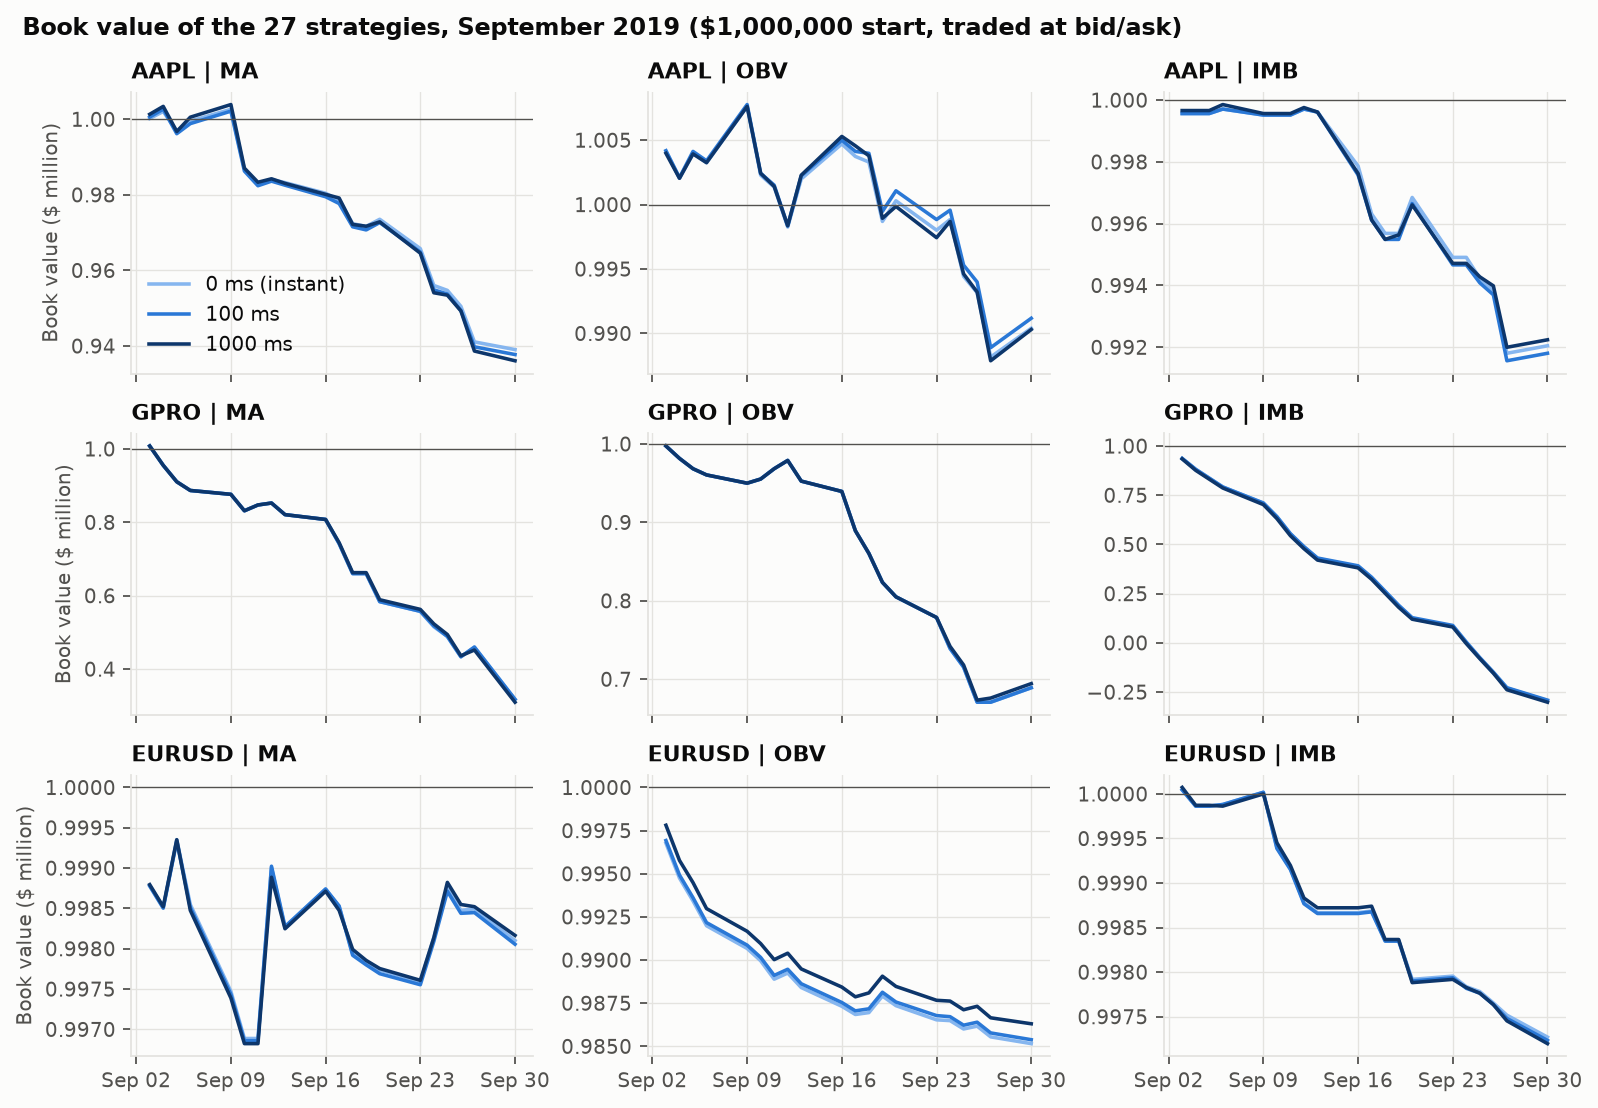
\includegraphics[width=0.92\textwidth]{figures/02_book_value_27_strategies.png}
  \caption{Book value of the 27 strategies over the month.}
\end{figure}

\begin{figure}[H]
  \centering
  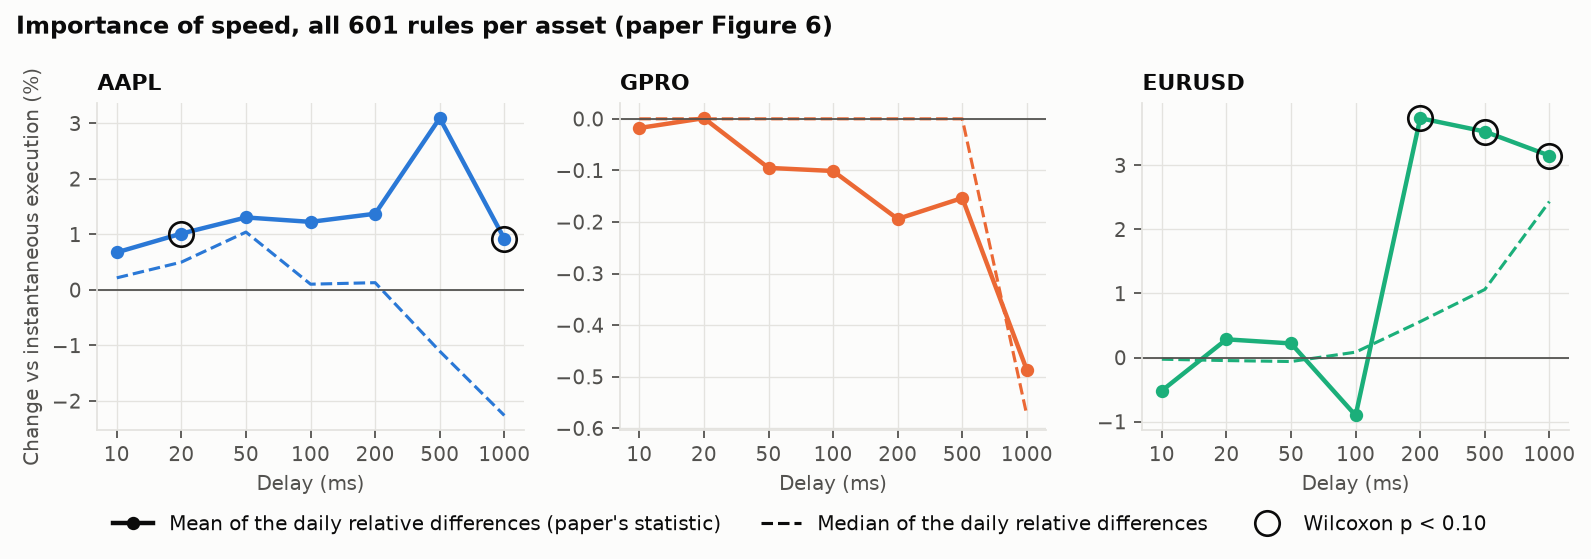
\includegraphics[width=\textwidth]{figures/04_importance_of_speed_all.png}
  \caption{Importance of speed for all rules, at the paper's seven delay levels.}
\end{figure}

\begin{figure}[H]
  \centering
  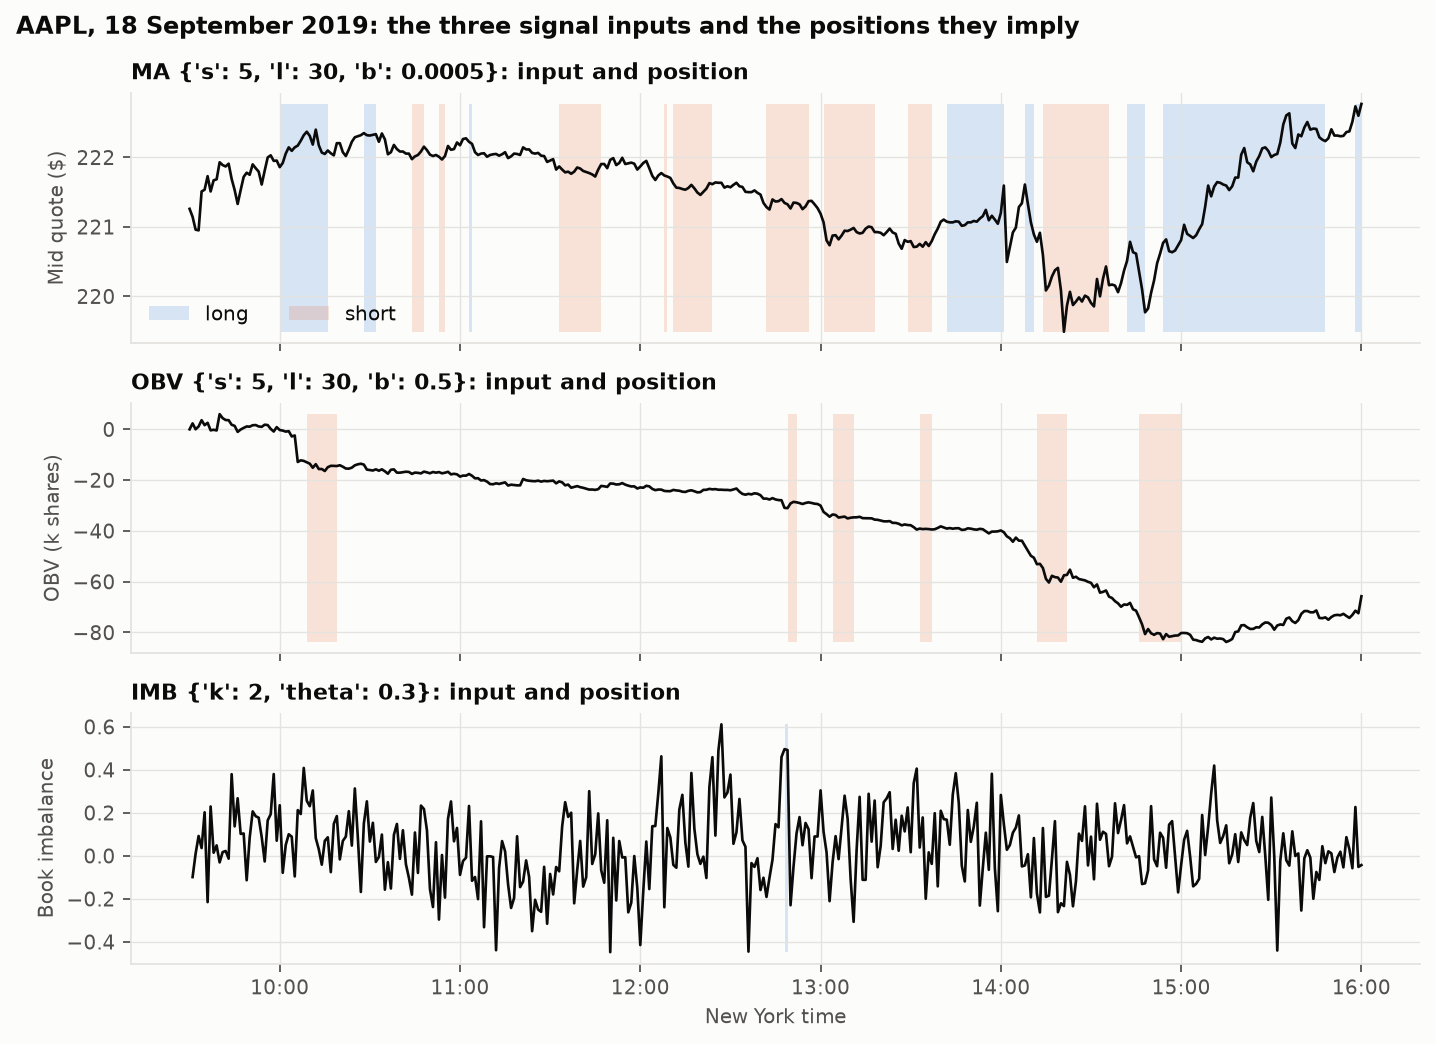
\includegraphics[width=0.85\textwidth]{figures/01_signals_example_day.png}
  \caption{The three signal inputs on AAPL on 18 September 2019 and the positions
  the baseline rules take.}
\end{figure}

\begin{figure}[H]
  \centering
  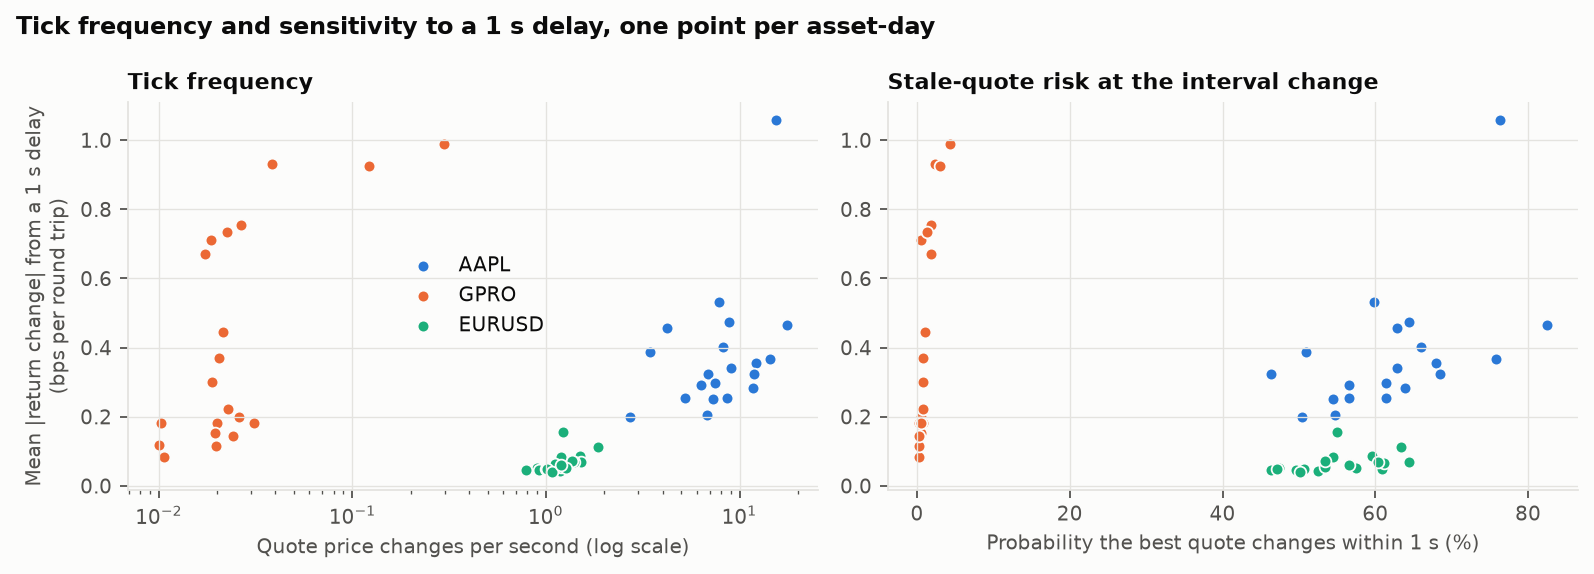
\includegraphics[width=0.9\textwidth]{figures/07_tick_frequency_vs_delay_sensitivity.png}
  \caption{Sensitivity to a 1 second delay against tick frequency, one point per
  asset-day.}
\end{figure}

\section{Appendix C. Code and reproduction}

Everything is in \texttt{Project/Part1\_Speed/} of the group repository.

\begin{itemize}[leftmargin=1.4em, itemsep=0.2em]
  \item \texttt{MFE230X\_project\_speed.ipynb}: the executed analysis, with every
        table and figure of this report.
  \item \texttt{src/speed.py}: data loaders, the three signals, the
        delayed-execution simulator, the random-rule test and the reporting
        functions.
  \item \texttt{src/download\_fx.py}: downloads the EUR/USD ticks.
        \texttt{src/report\_tables.py}: writes the tables of this report from the
        notebook's outputs.
  \item \texttt{data/}: the Databento and Dukascopy files. \texttt{outputs/}: the
        tables (CSV) and figures.
\end{itemize}

To reproduce: install \texttt{databento}, \texttt{jupyter}, \texttt{matplotlib},
\texttt{numpy}, \texttt{pandas} and \texttt{scipy}, then execute the notebook from
\texttt{Part1\_Speed/} (about two minutes).

\textbf{Reference.} M.~Scholtus and D.~van Dijk (2012), \emph{High-Frequency
Technical Trading: The Importance of Speed}, Tinbergen Institute Discussion Paper.

\end{document}
